%%% 3Background / %%%
\chapter{Background} \label{ch:background}
%To understand the interpretation of interaction graph and design of endorsement
%model, basic concepts about graph properties and metrics is required.
%Similarly, Blockchain relies a lot on cryptographic functions to maintain its
%property of the secure, immutable and attack-resilient structure. This chapter,
%therefore, provides a general overview of the background concepts that is
%required for the subsequent sections. 
Trust and reputation can be used across several domains, and their definitions
vary depending on context. It is essential to recognize the context in which
this term is being used. Similarly, blockchain can be seen as a relatively new
technology although the underlying sets of cryptographic functions it uses have
been around for a long time. Blockchain technology is being researched both by
academia and industry to explore its possibilities and in diverse use cases.
e.g., as a privacy-preserving smart contract~\cite{kosba2016hawk} or as a way
to protect personal data~\cite{zyskind2015decentralizing}. This chapter aims to
provide the necessary background theory by discussing the definition of trust
and reputation, blockchain technology and its components, cryptographic
functions, and graph properties in detail. 
%\section{Definition}
%This section aims to define trust and reputation as it exists and discuss the
%classification of its measure. Similarly, a brief overview of blockchain
%technology and its definition is presented. 
%Trust and reputation can have different meanings based on context. Similarly,
%blockchain still lacks a standard definition. As such, this section aims to
%provide a general introduction and definition that will be followed by this
%master's thesis project. 
\section{Trust and Reputation}
Trust encompasses a broad spectrum of domains and is context dependent.
Therefore, its definition varies based on context and discipline and as such
lacks collective consensus among researchers~\cite{mcknight1996meanings}.
Using the classification from McKnight et al., 1996~\cite{mcknight2001trust},
trust can be either Personal/Interpersonal, Dispositional or
Impersonal/Structural. Personal trust is when one person trusts another
specific person, persons, or things in a particular situation. Interpersonal
trust involves more than one trusting entities. i.e., two or more people (or
groups) trust each other. Dispositional trust refers to a more general trust
that is based on the personality attribute of the trusting party. i.e., an
entity is more likely to trust other entity based on their attitude and is
cross-contextual. While the trust mentioned above are implicitly directed
towards a person, impersonal/structural trust refers to the trust in
institutional structure. i.e., it is based on belief in regulatory enforcement
such as by contract law, judiciary systems rather than belief in involved
parties. \par

Trust can be generally seen as an entity's reliance on another interacting
entity to perform a specific set of the task given a specific situation.  As
pointed out by Gambetta et al.~\cite{gambetta2000can} ``Trust is the subjective
probability by which an agent assesses that other agent or group of agents will
perform a particular action that is beneficial or at least not detrimental.
"For an entity, $'A'$ to trust another entity ${'B'}$ or to evaluate $B's$
defined, \textit{reputation} is the perception of an individuals character or
standing. Like trust, reputation is context-dependent. e.g., Alice may be
trusted to answer linux questions efficiently but not windows related
questions~\cite{zacharia2000collaborative}. A significant difference between
trust and reputation is that the former takes the subjective measure as input
whereas the latter takes an objective standard (e.g., transaction history,
ratings) as an input to yield a resulting score that can aid in detecting
reliability/trustworthiness of an
entity~\cite{Sabater2005,castelfranchi2000trust}.\par 

Previous survey~\cite{ josang2007survey} has classified trust and reputation
measures as either subjective or objective measure. This classification is
further divided into specific or general. A subjective measure is based on an
individual's perspective and has no formal metrics. Specific, subjective
measures imply a subjective perception of an entity for a specific ability,
such as package delivery time of a seller or average response time. One way of
measuring this is via survey questionnaires that ask specific questions. On the
other hand, a general, subjective measure, aggregates all the individual scores
and provides an average standing of the user on the network. e.g., the
difference between positive and negative ratings used by eBay to give an
average rating. \par

An objective measure is used for product tests that can have some formal
criteria on which to rely on. e.g., hard disks can be measured based on
performance metrics such as transfer rate, access time, CPU usage. A specific,
objective measure takes an objective measure for a specific metric. i.e., how
good is a transfer rate for a particular hard disk whereas, a general,
objective measure accounts for all the relevant aspects and averages the
performance to give an average rating/score on a specific scale. \par

The table below shows the classification of trust and reputation measures as
discussed above based on~\cite{ josang2007survey}: 
%The classification of trust and reputation measures based on previous survey   
 \begin{center}\label{table:classificationTrust}
	\begin{tabularx}{\textwidth }{|X| X| X| }
		\hline
		 & Specific, vector-based & General, Synthesized \\
		 \hline
		Subjective & Survey questionnaires & eBay, voting \\
		\hline
		Objective & Product tests & Synthesised general score from product tests \\
		\hline
		\caption{Classification of trust and reputation measures.} 
	\end{tabularx}
\end{center}
\vspace{-15mm}
Individuals in online systems are identified by their online identities which
can be anything and not necessarily linked to their real-world identities.
Online identities play a crucial role in digital interaction and require
unknown entities to trust each other based on the reputation system of the
platform in use. Trust and reputation can be seen as a soft security mechanism
where it is up to the participants rather than the software/system to maintain
security. By definition, a security mechanism~\cite{stallings2017cryptography}
is a process (or a device incorporating such a process) that is designed to
detect, prevent, or recover from a security attack. Unlike hard security
mechanism such as access control, capabilities, authentication where a user can
be allowed or rejected access to the resource, reputation system do not provide
a method to block or detect a security attack directly. However, they define a
process to identify malicious users and avoid them from harming other users in
the system. Rasmusson, Lars and Jansson, Sverker~\cite{rasmusson1996simulated}
first used this term, to describe the idea of identifying malicious users and
preventing harm to other users in the context of secure open electronic
commerce. Reputation system needs to continuously receive feedback about the
user's behavior and maintain an updated record of users. It provides a way to
calculate the probability of success or risk of failure of a transaction
between interacting parties. 
%gather statistics on attacks, fraud data. 
%the trust value obtained in the endorsement network can be integrated with 
%existing reputation model of other transaction network and both combined 
%should give a higher accuracy for trustworthiness measure of entities(assumption)
\section{Cryptography} \label{sec:cryptography}
Cryptography offers algorithms to achieve confidentiality, integrity,
authenticity, and non-repudiation. Confidentiality and integrity ensure that
the information being communicated is not disclosed or has been modified to or
by any unauthorized parties. The data is hidden/encrypted such that only the
authorized parties can make sense out of it. i.e., decrypt using the previously
agreed upon key. Authenticity relates to confirming the truth of an attribute
claimed by an entity. Non-repudiation is associated with the property that any
entity who has previously sent the message cannot deny their
authorship~\cite{katz1996handbook}. \par 
A cryptosystem can be defined as a five-tuple $(P, C, K, E, D)$ where: 
\begin{itemize}
	\item $P$, is a finite set of plain texts.
	\item $C$, is a finite set of ciphertexts.
	\item $E$, set of encryption rules such that $e_{k}:P \Rightarrow C$
	\item $D$, set of decryption rules such that $d_{k}:C \Rightarrow P$ 
	\item For each $k \in K$, there is $e_k \in E$ and $d_k \in D$ such that $d_k(e_k(m)) = m$ for every plaintext $m \in P$.
\end{itemize}
A cryptosystem can be either symmetric or asymmetric. Symmetric makes use of
the same key for both encryption and decryption whereas asymmetric, also known
as public-key cryptography makes use of key pairs, public and private keys. The
public key can be publicly distributed, and an entity \textit{'A'} wishing to
send a confidential message to other entity \textit{'B'} can encrypt the
message using \textit{B's} public key $k_{p}$ to form ciphertext $c$. Upon
receiving $c$, \textit{B} can decrypt it using the private key $k_{s}$ that is
only known to \textit{B} and corresponds to the respective public key that was
used to form $c$. The computation of $k_{s}$ given $k_{p}$ is computationally
infeasible in a secure system. Besides public-key encryption, public-key
cryptography also has use in digital signature as discussed in
section~\ref{subsec:digitalsignature}. RSA~\cite{rivest1978method} is one example
of a public-private cryptosystem.

\subsection{Hash functions}
Cryptographic hash functions are one-way functions, also known as mathematical
trapdoor function that transforms an input message into a fixed length binary
output. It is one way because although converting a message input to a hash
value or a message digest can be done in constant time, reversing the operation
is practically impossible to achieve as it is computationally inefficient. An
important characteristics of hash function is its deterministic output. i.e.,
given an input, it will always produce the same output. This attribute
contributes to data verifiability as anyone can always verify if the produced
hash output for data matches by simply applying the data to the respective hash
function. \par 
Other significant properties of hash function that contributes to
reliability in digital security are~\cite{mironov2005hash}: 
\paragraph{One-way:} Given a key $k$, and an output $w$, it should be hard for
an attacker to find $x$ such that the hash of $x$ applied with $k$, produces
$w$.  ie., $H_k(x) = w$.
\paragraph{Second pre-image resistant:} Given a key $k$ and a string $x$, it
should be hard for an attacker to find $y$ such that $H_k(x)$ = $H_k(y)$. 
\paragraph{Collision-resistant:} Given a key $k$, it should be hard for an
attacker to find $x$ and $y$ such that $H_k(x) = H_k(y)$. \par   
%\begin{itemize}
%	\item One-way: Given a key k, and an output w, it should be hard for an
%		attacker to find x such that the hash of x applied with k, produces w.
%		ie., $H_k(x)$ = w.\\ 
%	\item Second pre-image resistant: Given a key k and a string x, it should
%		be hard for an attacker to find y such that $H_k(x)$ = $H_k(y)$.\\ 
%	\item Collision-resistant: Given a key k, it should be hard for an attacker
%		to find x and y such that $H_k(x)$ = $H_k(y)$. \\
%\end{itemize}
Earlier hash functions include MD5 which produced an output of size 128 bits.
Collision-resistant attack in MD5 is possible within seconds with a complexity
of $2^{39}$~\cite{wang2005break} MD5 operations. NIST published secure hashing algorithm (SHA)
in 1993 as the secure hash standard. Currently, SHA-3 is the latest in SHA
family of standards that was released in 2015 with SHA-0, SHA-1 and SHA-2 as
it's predecessor algorithms. Collision attack for SHA-1 was shown to be
practically pssible~\cite{stevens2017first} by creating two colliding pdf files
that produced same SHA-1 digest. It took equivalent processing power of 6,500
years of single CPU computation time and 110 years of GPU computation time.
Applications of hashing algorithms include digital signature, ISO checksums,
fingerprinting data etc. \par
These cryptographic hash functions are relevant in understanding blockchain
data structure. Merkle Tree~\cite{becker2008merkle,Berkeley} is a hash tree that is used
by blockchain to create a root hash of the list of transactions. Transactions
are explained in detail by section~\ref{sec:blockchain}. For understanding the
process of root hash creation, one can assume the list of transactions to be a
list of items. Assuming a binary tree of height $n$ with $2^{n}$ leafs, the
transactions are leaf nodes at height $0$. All the leaf nodes are paired and
hashed together. These hashes are again hashed together repeatedly until the
number of hash is only one. The final hash value is the hash of the root node
at height $n$. Figure~\ref{fig:merkleTree} illustrates the process of Merkle
root creation.
This root hash value is included as a block header and is significant for two
things in blockchain: 
\begin{figure}
	\begin{center}
		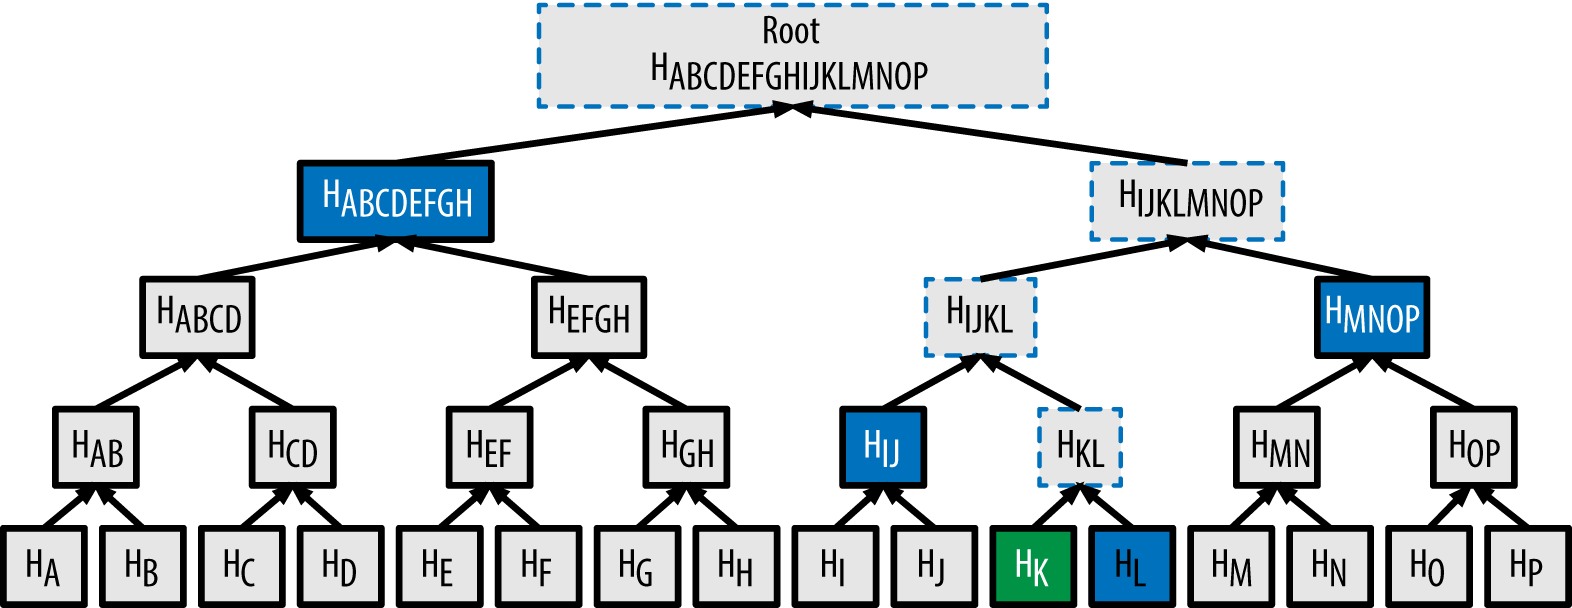
\includegraphics[width=0.8\textwidth]{Images/MerkleeTree.eps}
		\caption{Merkle root and data inclusion verification}
		\label{fig:merkleTree}
	\end{center}
\end{figure}
\begin{enumerate}
	\item Data integrity verification: An attempt to change any transaction data
		would completely change the root hash of the block.  
	\item Data inclusion verification: It is easy to verify the inclusion of a
		transaction in a block without requiring to include all the
		transactions. As shown in figure~\ref{fig:merkleTree}, the nodes
		labeled in blue are enough to verify the inclusion of transaction
		$H_{K}$. By looking at the root hash and the intermediate hashes, one
		can verify the inclusion of a specific data. The second
		preimage-resistance attribute ensures that the proof is not fake. 
\end{enumerate}

\subsection{Digital Signature} \label{subsec:digitalsignature}
A digital signature acts roughly like a physical signature in that the
signature can represent the identity and authorship of the signer. A digital
signature is a mathematical scheme that offers attribute such as authentication
(ability to prove that sender created the message) and non-repudiation (sender
cannot deny having sent the message). \par
The components of digital signature schemes are~\cite{rivest1978method}: 
\begin{itemize}
	\item Security parameter, $k$, chosen by user when creating public and
		private keys.
	\item Message, $M$, set of messages to which the signature algorithm is
		applied.
	\item Signature Bound, $B$, an integer bounding the total number of
		signatures that can be produced with an instance of signature scheme.
	\item Key generation algorithm, $G$, which any user $A$ can use to generate
		in polynomial time a pair $(P^{k}_A, S^{k}_A)$ of matching public and
		private keys. 
	\item Signature algorithm, $\sigma$, to produce a signature $\sigma(M,
		S_{A})$ for a message $M$ using the private key $S_{A}$. 
	\item Verification algorithm, $V$, to check that $S$ is a valid signature
		for a message $M$ using the public key $P_{A}$. i.e., $V(S,M,P_A)$ is only
		true if and only if the signature is valid. 
\end{itemize}
Two significant aspects of the digital signature scheme are signing algorithm
and verification algorithm. If Alice wants to send a signed message to Bob,
then she can create the signature using her private key and send the message
along with the signature to Bob. Bob can verify that the message originated
from Alice by using the verification algorithm on the signature using Alice's
public key. If the verification function returns true, then Alice cannot deny
having sent the message. Similarly, if the verification algorithm returns
false, then that would imply that the signature is invalid. \par   

In the context of the blockchain, if Alice wanted to send a value (transaction)
to Bob, the following steps would have to take place. Alice has to create a
transaction data structure with values for the required fields. Transaction
data and necessary fields are explained in detail by
section~\ref{sec:blockchain}. For this example, data can be Bob's address and
value that Alice wants to send to Bob. The data is serialized using the
underlying serialization algorithm. A hash function is then applied to this
serialized message. The signature on this hash value is created by using the
signature algorithm of the blockchain. In case of
ethereum~\footnote{https://www.ethereum.org/}, Alice would compute the ECDSA
signature. This signature (or the components) is appended to the transaction
and Alice can then submit this transaction over to the blockchain network. When
the transaction gets broadcasted, there are some special nodes
(miner/validator) that are supposed to pick this transaction and put it in a
block. After this happens, the transaction can be seen and verified by anyone
on the public blockchain network. If Bob or anyone wants to verify the
signature, they need to provide the signature, serialized transaction, and the
public key of Alice to the signature verification function. Alice can always
prove that she owns the public key because she owns the corresponding private
key that generated the signature. The transaction message is unalterable since
any modification to the message would refute the signature.  The explanation
above provides a high-level overview of the signing process.  Concepts such as
data serialization and transaction validation are discussed in detail by
section~\ref{subsec:consensus}.
%A digital signature acts as an intermediary to prove that an entity A, has the
%password without ever requiring A to reveal it. As discussed earlier,
%public-key cryptography uses key-pairs that correspond with each other. In
%context of blockchain, if Alice wants to send a value (transaction) to Bob, she
%can create a transaction message, sign it using her private key and broadcast
%the transaction over the network. Her signature and the transaction message
%will be publicly available on the network(assuming a public blockchain
%network). Anyone on the network can verify that the signature corresponds to
%Alice's public key. Thus, Alice can always prove that she is the owner of the
%public key from where the message originated. The signature is dependent on the
%message, and therefore any attempt to modify the message will refute the
%signature.
%figure showing basic process
%\section{Blockchain}\label{sec:blockchain}
%Blockchain can be defined as a distributed record of state changes that let
%anybody on the network audit state changes and prove with mathematical
%certainty that the transactions transpired according to the blockchain
%protocol. There exist several definitions of blockchain technology each
%specific to their closest use case. A formal standard definition of Blockchain
%is under development as ISO/TC 307~\cite{ISOTC307}.\\
%Vitalik Buterin, the founder of Ethereum, defines it this
%way~\cite{VitalikVisions}: "A blockchain is a magic computer that anyone can
%upload programs to and leave the programs to self-execute, where the current
%and all previous states of every program are always publicly visible, and which
%carries a very strong cryptoeconomically secured guarantee that programs
%running on the chain will continue to execute in exactly the way that the
%blockchain protocol specifies."\\
%\begin{quote}
%	\centering
%	"A blockchain is a magic computer that anyone can upload programs to and
%	leave the programs to self-execute, where the current and all previous
%	states of every program are always publicly visible, and which carries a
%	very strong cryptoeconomically secured guarantee that programs running on
%	the chain will continue to execute in exactly the way that the blockchain
%	protocol specifies."
%	\footnote{\url{https://blog.ethereum.org/2015/04/13/visions-part-1-the-value-of-blockchain-technology}} 
%\end{quote}
%This definition provides a broad overview of what blockchain does. As a
%continually developing discipline, it keeps adapting to a new definition while
%maintaining the essence. The major innovation of blockchain as an architecture
%is distributed, decentralized trustless (i.e., verification of transaction
%doesn't require a trusted third party or require transacting parties to trust
%each other) transactions~\cite{Bitcoin_Satoshi}. It completely removed the need
%for an intermediary trusted third party by building trust in the system itself.
%One dimension of trust as mentioned by ~\cite{miller2010trust} is trust in data
%which is based on integrity of stored data.  Trusting data ensures that the
%data is appropriate for use: accurate, precise, available, and
%uncorrupted~\cite{miller2010trust}.  Blockchain achieves this by use of
%cryptographic schemes mentioned in section~\ref{sec:cryptography}.
%assuring
%tamper-resistant, fault-tolerance, zero-downtime
%characteristics~\cite{swan2015blockchain}. 
% ~\cite{enoughBitcoinForEthereum}
\section{Blockchain Technology} \label{sec:blockchain}
Blockchain can be defined as a distributed record of transactions that lets
anyone on the network to audit the state changes and prove with mathematical
certainty that the transactions transpired according to the blockchain
protocol. There exist several ways to define blockchain, and every definition
is relevant to its specific use cases. A formal standard definition of
blockchain is under development as ISO/TC 307~\cite{ISOTC307}. There are
several blockchain platforms in operation today with varying design goals and
principles. Bitcoin~\cite{Bitcoin_Satoshi} is believed to be the first
application that made use of blockchain technology. However, the blockchain
applications and platform have evolved since then, and the current uses barely
show similarity to the first application. The purpose of bitcoin as the first
application was to have a P2P electronic cash system in an open, public,
distributed, decentralized and trustless environment. Trustless is a
significant attribute here because it completely removed the need for a trusted
intermediary. The idea of digital cash had been around since 1990 with
cryptographer David Chaum discussing untraceable electronic
cash~\cite{chaum1988untraceable}. However, bitcoin was able to solve the flaw
of a digital cash scheme, namely double spending problem. i.e., If $A$ had $10$
units of digital cash and sent it to $B$, then $A$ should have this amount
deducted from his account such that he is not able to spend the same amount
again. Bitcoin solved this problem without the use of trusted intermediaries
and without requiring participating entities to trust each other. Similarly, it
solved the Byzantine General's problem which is a problem in the distributed
computing environment where several agents need to agree on a state over an
unreliable network and without a trusted third party. \par
Examples of other platforms that extends bitcoin are
Namecoin~\footnote{https://namecoin.org/},
counterparty~\footnote{https://counterparty.io/}. Similarly,
ethereum~\cite{buterin2013ethereum} is a programmable blockchain platform that
offers a turing complete programming language~\cite{dannen2017introducing} and
allows anyone to write smart contracts and execute code to change the
blockchain state. Ethereum was considered to be suitable for this project for
its open source ecosystem and the availability of several test networks and
active community of developers with updated resources. Therefore, this master's
thesis project uses ethereum to write smart contracts and deploy the
application to the blockchain network. Examples of private blockchain
platforms are hyper ledger
fabric~\footnote{https://www.hyperledger.org/projects/fabric/},
Multichain~\footnote{https://www.multichain.com/} etc.\par
Blockchain technology is a variant of a distributed database implemented on a
P2P network. Every participating node in the network has the same copy of the
history of records of the database. It is essentially a chain of blocks, as the
name suggests. Each block consists of a list of transactions and the ordering
of block shows the time at which the particular block was added to the chain.
The data structure of blockchain is analogous to singly linked list with each
blocks having a hash value pointing to the previous block. \par
\paragraph{Transactions:} Transactions are signed messages that can be
submitted by the originator and are collected and stored on blockchain network
by miners. Miners are special nodes that have the computational resource to add
transactions to the block. Miners collect the list of unconfirmed transactions
(transactions that are submitted but not yet added to the block),finds the root
hash of all transactions and attempts to find the solution to the cryptographic
puzzle (e.g., Proof-Of-Work). The process of finding the hash value is given in
section~\ref{subsec:consensus}.

%Blockchain technology is a variant of distributed database implemented on a P2P
%network. Every participating node in the network has the same copy of history
%of records of the database. Blockchain is essentially a chain of blocks, as the
%name suggests. Each block consists of list of valid transactions (signed
%messages) collected by validators/miners of the network. The linking and
%ordering of transactions are also the responsibility of validators. The
%validators propose a block they have unlocked to the network which can either
%be accepted or rejected. If accepted, the newly created block gets linked to
%the existing blockchain with a hash pointing to the previous block. As such,
%blockchain provides the transaction ordering that every node agreed on at a
%given time. Consensus metric helps to establish and maintain the integrity of a
%blockchain
%system~\footnote{https://github.com/ethereumbook/ethereumbook/blob/develop/consensus.asciidoc}.
%The primary attributes that constitute a blockchain system are distributed,
%decentralized and time-stamped transactions.  There have been P2P protocols
%deployed as a file-sharing or other form of content delivery services before
%Blockchain. What makes Blockchain stand out from them is, for the first time,
%it makes it possible to transfer values online on a P2P network without a
%double-spending problem, i.e., if a peer \textit{'A'} sends a file or a value
%\textit{'v'} to \textit{'B'}, then the file should be owned by \textit{'B'} and
%removed from the account of \textit{A}. \textit{'A'} should not be able to send
%the same file \textit{'v'} to other entities on the network. This was the
%significant contribution of the technology. 
%While, transferring digital contents, sharing information were
%possible before, transferring values was made possible by Blockchain
%technology.
%~\cite{pilkington201611}
%\subsection{Basic Concepts}
%transaction, message, signature, broadcast, verify, network, miners, validate, write blocks 
\subsection{Evolution \& Categories}
Along the dimension of validation and access control~\cite{voronchenko2017you},
Blockchain can be categorized as a public permissionless system, public
permissioned, and private permissioned. 
\begin{itemize}
	\item Public Permissionless: Anyone can join the network and become a writer
		of the block as long as they can solve a problem or reach the consensus
		that satisfies the underlying protocol. The records are publicly
		available and thus publicly verifiable. 
	\item Public Permissioned: Anyone can still join the network, but a writer
		of the block is known but not necessarily a trusted entity. The records
		are publicly verifiable. 
	\item Private Permissioned: This is similar to the Public permissioned
		setting, but the records are not made public and therefore doesn't
		offer public verifiability. This kind of setup is more specific to
		business use-cases where one business does not need to know about other
		business policies or customer information etc. 
\end{itemize}
%~\cite{voronchenko2017you} provides a detailed discussion on various blockchain
%types and their uses.
\subsection{Consensus Mechanisms}\label{subsec:consensus}
As a distributed database with multiple writers, there has to be a way for
everyone to reach a consensus on a shared global view of the network. Consensus
mechanisms allow doing so. Based on consensus mechanisms, systems can be
distinctly categorized into~\cite{HashgraphConsensusCategory}:
\paragraph{Leader Based System:} In this case, there is a pre-selected leader
that collects all the transactions and appends new records to the blockchain.
Having a small group or consortium, it has low computational requirements. As a
blockchain protocol, it offers an immutable audit of the records. However, just
like any other centralized system, this system is susceptible to DDOS attacks
and third-party (leader) interference. Generally used in a private or
permissioned blockchain setup, it offers higher throughput compared to public
permissionless blockchains. Examples include Hyperledger Fabric, R3 Corda etc. 
\paragraph{Proof-Of-Work (PoW):} This is the most widely used consensus
mechanism in a public permissionless setup. As the name suggests, a
validator/miner needs to provide the proof to the network that it has done a
significant amount of work. This work requires miners to invest a substantial
amount of computational resources. The reason for this is that everyone (all
miners) compete to be the writer of the next block for which they need to solve
a cryptographic puzzle. Figure~\ref{fig:cryptographicPuzzle} shows the process of
finding a valid hash value. The miners are supposed to find a specific nonce
value which when concatenated with the transaction data should output a hash
value that is less than the target value. The target value keeps changing to
maintain a normal distribution of average block time. The nonce keeps
incrementing until the output hash satisfies the function requirement. Thus,
they have to compute many hash operations before finding the valid hash. When a
valid hash is found, then the miner gets to add the block to the existing chain
of blocks. All the blocks in the blockchain are formed by same process except
for genesis block. Genesis block is the first block in the blockchain and
therefore has no pointer to previous block. Examples include Bitcoin, Ethereum.
\begin{figure}
	\begin{center}
	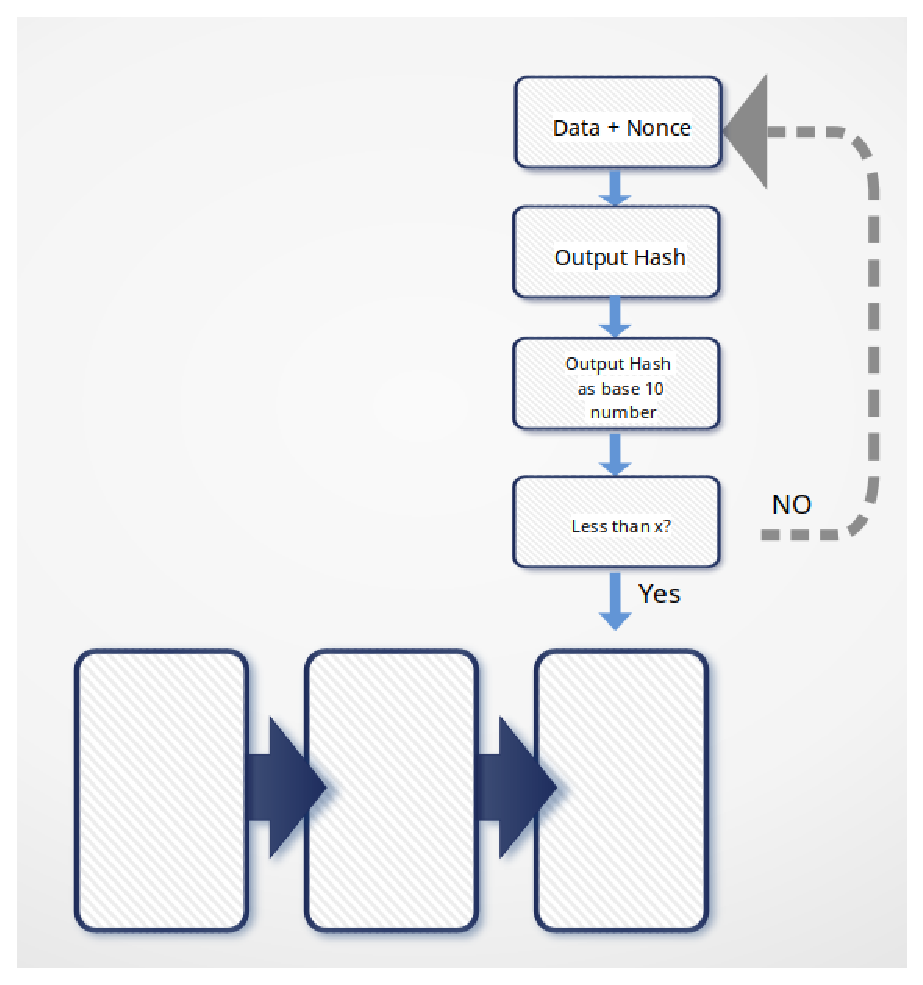
\includegraphics[width=0.5\textwidth]{Images/CryptographicPuzzle.eps}
	\caption{Cryptographic Puzzle}
	\label{fig:cryptographicPuzzle}
	\end{center}
\end{figure}
The apparent advantage of such consensus mechanism is that it makes the
system DDOS resistant while offering immutable audit trail and
scalability.  However, miners can still decide upon the order of
transactions to include in the block although they cannot modify the
transaction. As such, one could term this as 'unfair', since the
transaction does not get picked up in order of when it was broadcasted
to the network. 
\paragraph{Economy based systems:} Consensus mechanisms such as Proof-of-stake
or delegated proof-of-stake can be seen as an economy based system. Unlike PoW,
miners do not compete with each other to be the writer of next block thus
saving lots of computational resources. The general idea is that participants
can put the respective platform based native token they own at stake to
validate a block. Whoever has the highest value at stake gets to write the next
block. If the participation turned out to be a malicious one, then all the
tokens that were at stake get lost. As such, it puts scarce resource at stake.
However, this includes problem such as nothing-at-stake~\cite{houy2014will},
i.e., a node could vouch for two forks of the same blockchain with nothing to
lose. Other drawbacks of this approach are that there is no certainty of
consensus, and often has no total ordering of transactions, Examples include
Casper etc. 
%The PoW consensus mechanism, relies on SHA-256 hash (in Bitcoin)
%applied to the block header and nonce to produce a verifiable fingerprint of
%data. This is discussed in more detail in~\ref{sec:blockchain}. Proof-of-work
%was originally used in 1997 by Adam Back as a anti-spam system for the then
%proposed Hashcash~\cite{back2002hashcash}. The general idea being that the
%sender of message would have to compute some number of sha operations before
%sending the message.  The generated fingerprint could be checked by anyone to
%see if the sender has actually done the required number of computations. If a
%legitimate user sending out one email had to spend 'x' seconds to do the sha
%operations, a malicious user intending to send thousands of emails had to spend
%1000x seconds. \\
\subsection{Smart contracts}
A contract in a classical sense is a set of rules with pre-defined obligations
and permissions that participants are assumed to follow. It does not
necessarily need to be legally binding or even associated with the outside
world. The term Smart contact was first coined by Cryptographer Nick Szabo, in
1994~\cite{SzaboSmart1994} and defined as a computerized transaction protocol
that can execute the terms of a contract. Szabo points out that the contract
design should fulfill four objectives~\cite{szabo1996smart}: \\
%\footnote{https://universe.ida.dk/media/23422289/fritz-henglein.pdf}.
\begin{itemize}
	\item \textbf{Observability}, ability to observe the contract, performance of
		principal(agents who have agreed to the contract) and prove their
		performance.\\
	\item \textbf{Verifiability}, the ability of principals to prove to the
		arbitrators that the contract has been performed or breached. \\ 
	\item \textbf{Privity}, to ensure that the third party should not have
		control or knowledge of the content or performance. It correlates to
		both privacy and confidentiality of principals of contract and the
		contract itself. \\
	\item \textbf{Enforceability}, to make the contract self-enforcing which
		can be attributed to by verifiability, built-in incentives mechanism,
		and objectives mentioned above. \\
\end{itemize}
Privity refers to minimization of third-party vulnerability by limiting
knowledge and control whereas, on the other end, observability and
verifiability demands invoking it to an extent. As such, a trade-off is
required wherein an optimal balance between these objectives should meet. Thus,
trusted intermediaries were introduced with minimal control/observability.
However, privity was not guaranteed in case of
dispute~\cite{szabo1997formalizing}. Following the invention of Bitcoin and
several decentralized blockchains, the definition of smart contracts have
evolved. Ethereum being the first platform to offer programmable blockchains,
introduced a virtual machine, EVM (Ethereum Virtual Machine), where the
contract code can be executed that results in a deterministic output provided
the same transaction context and blockchain
state~\cite{MasteringEthereum}}.
EVM often referred to as a single world computer, runs on every ethereum node
and given the same initial state produces the same final state. Several high
level languages can be used to write smartcontracts for different blockchain
platforms. Examples include solidity, serpent, LLL, etc.  For the sake of
relevance to this project, solidity as the smart contract language and Ethereum
as the blockchain will be used as a point of view henceforth. Contract's code
resides in the blockchain as an immutable form.  They are not autonomous
self-executing programs but rather needs to be called by a transaction or
invoked by other contracts. Once the code is registered and deployed on the
blockchain, its code cannot be altered by anyone, including the owner of the
contract. However, a possibility to include a killable function by the owner
exists which when called executes an EVM opcode called SELFDESTRUCT. This
deletes the contract from the blockchain. As in any Turing-complete language,
solidity is affected by the halting problem.  To address this, Ethereum
introduces the concept of gas. To store any state, or execute any operation,
gas needs to be supplied. Thus, a program that has a bug or a non-terminating
intention will eventually run out of gas and stop~\cite{whataresmartcontracts}.

\section{Reputation systems}
The most known internet reputation is assumed to be that of
eBay~\cite{resnick2002trust}~\footnote{https://www.ebay.com/}. It uses a
feedback based rating system where a user can rate a transaction along with
some textual feedback. The range of values used being \{1, 0, -1\}, positive,
neutral and negative respectively. The final aggregated score is computed by
subtracting the total of positive and negative ratings. This system could be
judged as working based on the sales volume and the observation that more than
half the buyers usually engage in providing feedback~\cite{resnick2006value}.
However, there are various issues of an online interaction system that this
method fails to address such as: 
\paragraph{Sybil Attack:} A user (buyer/seller) can create multiple
accounts(sybil identities) and give enough positive feedback to their original
account to inflate one's reputation.  Similarly, they can also provide multiple
negative feedbacks to any merchant and damage their reputation.
\paragraph{Inactive participation:} Users are more likely to provide feedback
for a satisfactory transaction and ignore a bad deal. Since the system is not
anonymous, it is possible to trace the sender of received feedback. Therefore,
users are more likely to fear retaliation from giving negative feedback.
\paragraph{Whitewashing:} The overall trust score of an entity is the
difference between positive and negative ratings received in total. As such, an
account can have a significant negative value. In which case, it is more
beneficial to start afresh with a new account then to recuperate the account
with poor reputation scores.

Other online systems that make use of similar reputation mechanism based on
votings/ratings are StackExchange~\footnote{https://stackexchange.com/},
yelp~\footnote{https://www.yelp.com/}, Quora~\footnote{https://www.quora.com},
Reddit~\footnote{https://www.reddit.com/}. Most of the online interaction
system (e.g., e-commerce, Q\&A platform) employ a client-server architecture
which lets a central entity in control of stored data. The centralization of
data management has both pros and cons to it. While it makes the network simple
to filter out malicious content from being served, it also acts as a single
point of failure. On the other hand, distributing data from a P2P system where
any nodes on the network can serve contents solves this issue of central point
of failure. The distributed nature of a P2P system also makes it more
straightforward to distribute malicious contents over the network. The peer
requesting a file can have it served from any participating node. If the
content of this file is malicious, then it is more likely to spread faster in a
P2P network than a centralized system. Therefore, a reputation management
system that can work in a distributed and decentralized environment is
significant for P2P systems such as file-sharing, content delivery
applications, etc. for detecting the quality of file/content or the owner of
those files. In light of this, researches and proposals on decentralized
reputation methods have been performed, few of which are discussed below.\\ 

\subsection{Graph properties}
A graph, as the name suggests can be used to represent objects and their
relationships graphically. \par
Formally, a graph~\cite{bondy1976graph}, $G$, is an ordered triple $(V,E,\phi,
G)$ where:
\begin{itemize}
	\item $V$ is a non empty set of vertices $v$.
	\item $E$ is a non empty set of edges $e$.
	\item $e$ connects two vertices, where, $v \in V$ and $e \in E$.
	\item $\phi_G$ is an incidence function that assigns pair of vertices to
		each edge of graph $G$. 
	\item $\phi_G(e) = uv$ represents that e is an edge that joins vertices $u$
		and $v$.
\end{itemize}
Based on these properties, any online interaction system can be modeled
graphically including reputation system. Each node on the network can represent
agents/users that interact with other users. This interaction can represent the
relationship between nodes as the edges connecting vertices. The transfer of
data between the nodes can be quantified to represent the weight of the edge.
This weight value can be used to determine the strength or weakness of
relationship between the nodes. Modeling the interaction as a graph can help to
understand and analyze its complexity at different levels. By observing the
local properties of a particular node such as its activity, connection degree,
its neighbors, and interactions, one can derive useful information about a
node. Similarly, the node’s relative position in a given graph can help to
determine its centrality and connectivity. An overall structure of the network
(graph topology) can help to study the global properties of the graph. \par
Network metrics that are helpful in analyzing the complexity of interactions at
different levels~\cite{gkorou2014exploiting} and used for evaluation of results
in this project are:
\paragraph{Degree Connectivity:} The number of connections a node has is the
degree of its connec- tivity. The number of inflow is referred to as indegree
whereas the number of outflows is the outdegree of a node. Usually, a higher
degree of connectivity implies a higher likelihood for information (relevant
data to the network) to pass through that node.  

\paragraph{Network Centrality:} Centrality refers to the significance of a node
in the network. i.e., how important the node is in the overall network. The
degree of connectivity is one way to measure centrality of a node. Similarly,
there are other centrality measures which includes: Closeness centrality,
Betweenness centrality, Prestige centrality.
\paragraph{Closeness Centrality:} refers to how close a node is to other nodes
in the network.
\paragraph{Betweenness Centrality:} refers to the number of nodes to which the
given node acts as a connector. i.e., how many nodes passes through this node.
\paragraph{Prestige Centrality:} refers to the significance of the node based
on the significance of the adjacent nodes(nodes one is connected to). To
observe and analyze the behavior at the macro-level, one needs to look at the
overall structure of the graph. i.e., Network topology that shows how
constituent parts are interconnected to form the graph as a whole. They can
form ring, star, tree, or mesh structure or be a fully connected graph where
each node are connected to each other.









%\subsection{Ethereum specific concepts}



%\subsection{Applications}




